\documentclass[conference]{IEEEtran}
\usepackage{cite}
\usepackage{amsmath,amssymb,amsfonts}
\usepackage{graphicx}
\usepackage{textcomp}
\usepackage{xcolor}
\usepackage{url}
\usepackage{listings} % include code
\usepackage{hyperref} % clickable refs
\def\BibTeX{{\rm B\kern-.05em{\sc i\kern-.025em b}\kern-.08em
    T\kern-.1667em\lower.7ex\hbox{E}\kern-.125emX}}

% pretty box for takeaways
\usepackage{tcolorbox}
\newcommand{\takeaway}[1]{%
\begin{tcolorbox}[colframe=black,boxrule=0.5pt,arc=4pt,
      left=6pt,right=6pt,top=6pt,bottom=6pt,boxsep=0pt,width=\columnwidth]%
      {Takeaway: #1}
\end{tcolorbox}%
}

% acronyms
\usepackage{acronym}
\newacro{ip}[IP]{Internet Protocol}
\newacro{dns}[DNS]{Domain Name System}

\begin{document}

\title{Paper Title}

\author{\IEEEauthorblockN{Given Name Surname}
\IEEEauthorblockA{\textit{dept. name of organization (of Aff.)} \\
\textit{name of organization (of Aff.)}\\
City, Country \\
email address}
\and
\IEEEauthorblockN{Given Name Surname}
\IEEEauthorblockA{\textit{dept. name of organization (of Aff.)} \\
\textit{name of organization (of Aff.)}\\
City, Country \\
email address}
}

\maketitle

\begin{abstract}
    Abstract text

\end{abstract}

\begin{IEEEkeywords}
    key, words
\end{IEEEkeywords}

\section{Introduction} \label{sec:introduction}
The \ac{dns}~\cite{RFC1034,RFC1035} translates human-readable 
domain names to \ac{ip} addresses.

\section{Background} \label{sec:background}

\begin{figure}[!h]
    \centering
    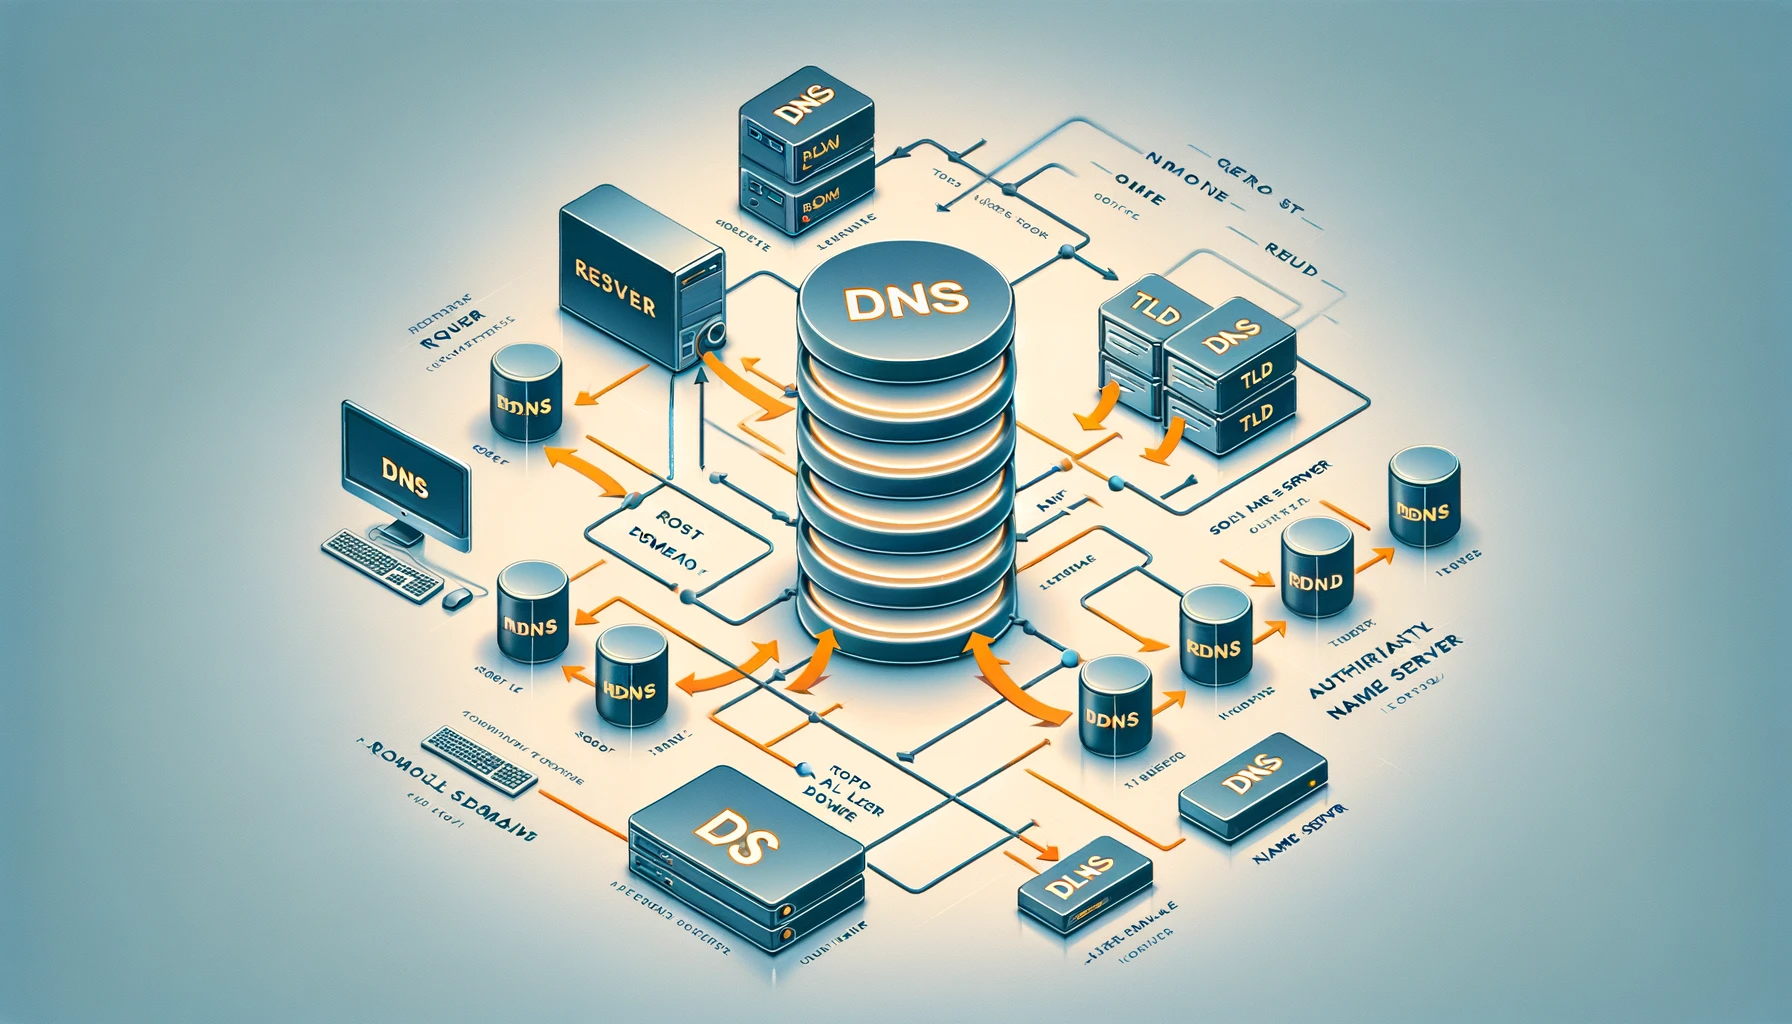
\includegraphics[width=.5\textwidth]{img/dns.png}
    \caption{An AI generated image of DNS}
    \label{fig:dns}
\end{figure}

\ac{dns} is a complex system (see Figure~\ref{fig:dns}).


\section{Method} \label{sec:method}
The function of \ac{dns}, as described in Section~\ref{sec:background}...

\section{Measurements} \label{sec:measurements}
Measurement text

\subsection{First Measurement} \label{sec:measurements:first}
Results
\takeaway{We found that...}

\subsection{Second Measurement} \label{sec:measurements:second}
Results
\takeaway{We found that...}

\section{Discussion} \label{sec:discussion}
Based on our findings in Section~\ref{sec:measurements}...

\section{Related Work} \label{sec:relatedwork}
Other studies have done similar work...

\section{Conclusion} \label{sec:conclusion}
We have done the following and found that...


\bibliographystyle{plain}
\bibliography{src/ref} 

\end{document}
